\documentclass[]{article}
\usepackage{tikz}
\usetikzlibrary{shadings, shadows, shapes, arrows, calc, positioning, shapes.geometric}
\usepackage{pgfplots}
\pgfplotsset{compat=1.16}
\usepackage{mathtools,amssymb}
%\input{Preamble}
%\input{(SpecialDistanceCourse}
%\input{FRAMES}
\begin{document} 
% \chapter{Gather Newer Results and Figures}
\section{What is this document?}
%  Figure template at bottom
We are collecting new figures to discuss and possibly use. 

\subsection{Link on and off - with changed CG }

\begin{figure}[h!tb] \centering    
    \begin{tikzpicture}
    %\draw[step=1.0,black,thin] (-4,-5) grid (4,5);
        \node[inner sep=.5pt] (plain) at (0,0)
            {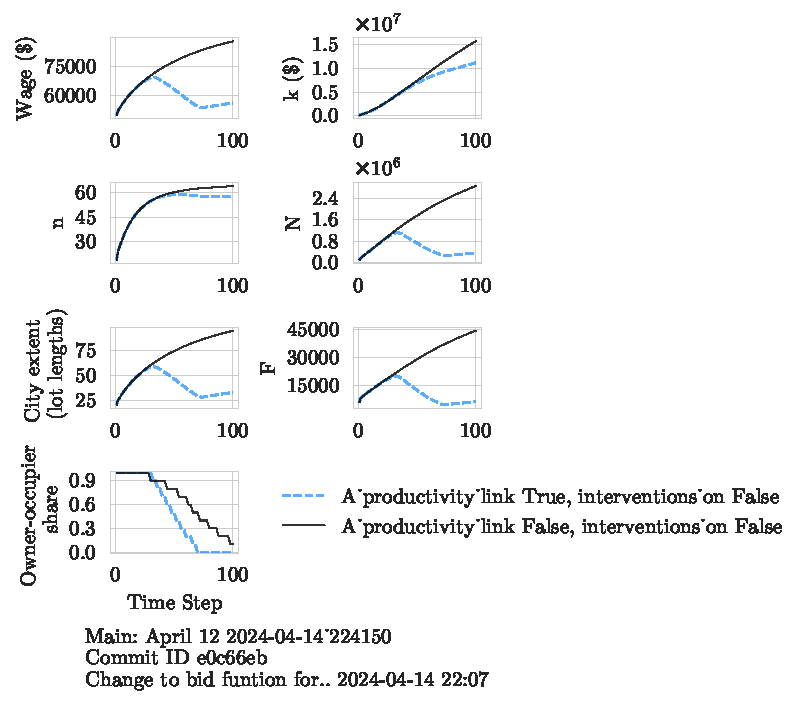
\includegraphics[height=10cm,trim={.2cm 1.4cm 5cm 0},clip]
            {31-fig/link-on-off_224150.pdf}};  
    % White box
        \begin{scope}[shift={(1.2,-4.05)}]
            \draw[color=white, fill=white, fill= white] (0,0) 
            rectangle (2.8,1.5);   %, fill=white]
            \node at (2.5,1.05)[align=left, text width=4cm, scale=01.2]
                {\tiny productivity link on};
            \node at (2.5,.58)[align=left, text width=4cm,  scale=01.2]
                {\tiny No link};
        \end{scope}
    \end{tikzpicture}
      \caption{}
\label{fig:newlink-on-off}
\end{figure}
Figure~\ref{fig:newlink-on-off} shows the effect of the productivity linkage with the new bidding formula.  The impacts are as before, but housing is  financialized more completely with and without linkage  than with the old formulation.
%%%%%____________________
\subsection{Link on and off  and 3 CGTI values - with changed CG }
Figure~\ref{fig:newlinkon-off-CGTI } shows


\begin{figure}[h!tb]  \centering
    \begin{tikzpicture}
%\draw[step=1.0,black,thin] (-4,-5) grid (4,5);
        \node[inner sep=.5pt] (plain) at (0,0)
            {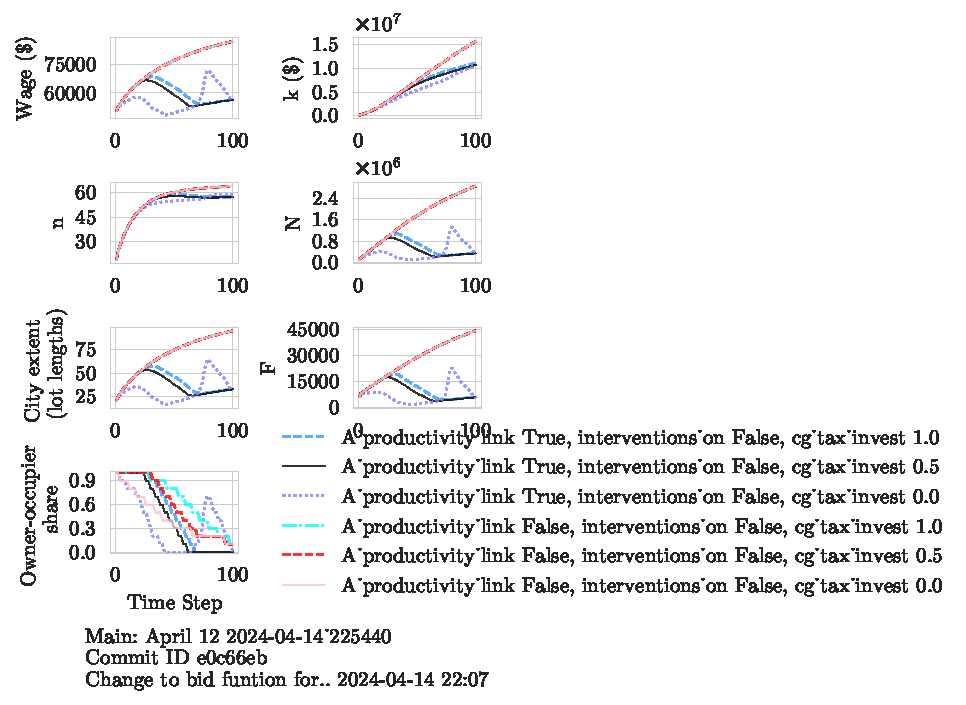
\includegraphics[height=10cm,trim={.2cm 1.4cm 7.5cm 0},clip]
            {31-fig/link-on-off-cg_tax_i_0-pt5-1225440.pdf}}; 
            
        \begin{scope}[shift={(1.2,-5.07)}] % White box for labels
            \draw[color=white, fill=white, fill= white] (0,-2) rectangle (2.8,3.3);   %, fill=white]
            \node at (2.5,3.05)[align=left, text width=4cm, scale=01.2]
                {\tiny link + 100\% capital gains tax};
            \node at (2.5,2.55)[align=left, text width=4cm, scale=01.2]
                {\tiny link + 50\% capital gains tax};
            \node at (2.5,2.1)[align=left, text width=4cm, scale=01.2]
                {\tiny link + zero capital gains  tax};
            
            \node at (2.5,1.6)[align=left, text width=4cm, scale=01.2]
                {\tiny no link + 100\% capital gains tax};
            \node at (2.5,1.15)[align=left, text width=4cm, scale=01.2]
                {\tiny no link + 50\% capital gains tax};
            \node at (2.5,.7)[align=left, text width=4cm, scale=01.2]
                {\tiny no link + zero capital gains  tax};
        \end{scope}
    \end{tikzpicture}
          \caption{link-on-off-CGTI }
\label{fig:newlinkon-off-CGTI }
\end{figure}

Figure~\ref{fig:newlink-on-off} shows three capital gains taxes on investors  with and without the productivity. (link-int-cg\_tax-0-pt5-1\_221736.pdf, which is in the 31-fig folder  shows three capital gains taxes on investors  without the productivity. The results agree). All three no-link cases follow the highest trajectory for wage and population, but somewhat different ownership paths. 

With linkage, higher capital gains taxes result in slower takeover of the housing market by financial players, the lowest capital gains tax on investors does the most damage and does that damage most quickly. It also appears to generate cycling behaviour that might be interesting to examine in a longer run.

% \subsection{}
%Figure~\ref{ } shows

% \begin{figure}[h!tb] \centering
    %\begin{tikzpicture}
    %   %\draw[step=1.0,black,thin] (-4,-5) grid (4,5); 
        %\node[inner sep=.5pt] (plain) at (0,0)
    %     {\includegraphics[height=10cm,%width=.5\textwidth,trim={.2cm 1.4cm 7.5cm 0},clip]
   %      {NewFig/XXX.pdf}}; 
        % \begin{scope}[shift={(1.2,-4.05)}]
        %     \draw[color=white, fill=white, fill= white] (0,0) 
        %     rectangle (2.8,1.5);   %, fill=white]
        %     \node at (2.5,1.05)[align=left, text width=4cm, scale=01.2]
        %         {\tiny productivity link on};
        %     \node at (2.5,.58)[align=left, text width=4cm,  scale=01.2]
        %         {\tiny No link};
        % \end{scope}
    % \end{tikzpicture} 
    % \caption{link-on-off-CGTI }
% \label{fig:new1}
% \end{figure}




\end{document}